% math0 manuscript. Build with: latexmk -pdf paper.tex
\documentclass[11pt]{amsart}
\usepackage[margin=1.1in]{geometry}
\usepackage{amsmath,amssymb,amsthm,mathtools}
\usepackage{url}
\usepackage{hyperref}
\usepackage{xcolor}
\usepackage{listings}
\usepackage{newunicodechar}
\usepackage{tikz}

\lstdefinelanguage{lean}{
  keywords={theorem,lemma,def,abbrev,example,fun,by,have,show,from,let,in,if,then,else,match,with,
    namespace,end,open,import,section,variable,instance,structure,where,calc,obtain,intro,exact,
    refine,rcases,rintro,simp,omega,decide,norm_num,linarith,nlinarith,positivity,induction,cases,
    private,noncomputable,ring,push_cast,set,unfold,convert,rw,congr,linear_combination},
  sensitive=true, comment=[l]{--}, morecomment=[s]{/-}{-/}, string=[b]"}
\lstset{language=lean, basicstyle=\ttfamily\footnotesize, columns=fullflexible, keepspaces=true, breaklines=true,
  keywordstyle=\color{blue!60!black}\bfseries, commentstyle=\color{gray}, frame=single,
  extendedchars=true, inputencoding=utf8,
  literate={ℕ}{{$\mathbb{N}$}}1 {ℤ}{{$\mathbb{Z}$}}1 {ℝ}{{$\mathbb{R}$}}1 {ℂ}{{$\mathbb{C}$}}1
    {∀}{{$\forall$}}1 {∑}{{$\sum$}}1 {↔}{{$\leftrightarrow$}}1 {¬}{{$\neg$}}1 {∧}{{$\wedge$}}1
    {→}{{$\to$}}1 {←}{{$\leftarrow$}}1 {≤}{{$\le$}}1 {≠}{{$\ne$}}1 {⟨}{{$\langle$}}1 {⟩}{{$\rangle$}}1
    {·}{{$\cdot$}}1 {ζ}{{$\zeta$}}1 {Φ}{{$\Phi$}}1 {σ}{{$\sigma$}}1 {α}{{$\alpha$}}1}
% Unicode commonly found in Lean sources.
\newunicodechar{ℕ}{\ensuremath{\mathbb{N}}}
\newunicodechar{ℤ}{\ensuremath{\mathbb{Z}}}
\newunicodechar{ℚ}{\ensuremath{\mathbb{Q}}}
\newunicodechar{ℝ}{\ensuremath{\mathbb{R}}}
\newunicodechar{ℂ}{\ensuremath{\mathbb{C}}}
\newunicodechar{∀}{\ensuremath{\forall}}
\newunicodechar{∃}{\ensuremath{\exists}}
\newunicodechar{→}{\ensuremath{\to}}
\newunicodechar{←}{\ensuremath{\leftarrow}}
\newunicodechar{↔}{\ensuremath{\leftrightarrow}}
\newunicodechar{↦}{\ensuremath{\mapsto}}
\newunicodechar{¬}{\ensuremath{\neg}}
\newunicodechar{∧}{\ensuremath{\wedge}}
\newunicodechar{∨}{\ensuremath{\vee}}
\newunicodechar{≤}{\ensuremath{\le}}
\newunicodechar{≥}{\ensuremath{\ge}}
\newunicodechar{≠}{\ensuremath{\ne}}
\newunicodechar{∈}{\ensuremath{\in}}
\newunicodechar{∉}{\ensuremath{\notin}}
\newunicodechar{⊆}{\ensuremath{\subseteq}}
\newunicodechar{∩}{\ensuremath{\cap}}
\newunicodechar{∪}{\ensuremath{\cup}}
\newunicodechar{∑}{\ensuremath{\sum}}
\newunicodechar{∏}{\ensuremath{\prod}}
\newunicodechar{⟨}{\ensuremath{\langle}}
\newunicodechar{⟩}{\ensuremath{\rangle}}
\newunicodechar{·}{\ensuremath{\cdot}}
\newunicodechar{∘}{\ensuremath{\circ}}
\newunicodechar{⁻}{\ensuremath{^{-}}}
\newunicodechar{¹}{\ensuremath{^{1}}}
\newunicodechar{²}{\ensuremath{^{2}}}
\newunicodechar{₀}{\ensuremath{_{0}}}
\newunicodechar{₁}{\ensuremath{_{1}}}
\newunicodechar{₂}{\ensuremath{_{2}}}
\newunicodechar{α}{\ensuremath{\alpha}}
\newunicodechar{β}{\ensuremath{\beta}}
\newunicodechar{ε}{\ensuremath{\varepsilon}}
\newunicodechar{δ}{\ensuremath{\delta}}
\newunicodechar{π}{\ensuremath{\pi}}
\newunicodechar{σ}{\ensuremath{\sigma}}
\newunicodechar{φ}{\ensuremath{\varphi}}
\newunicodechar{ζ}{\ensuremath{\zeta}}
\newunicodechar{Φ}{\ensuremath{\Phi}}
\newunicodechar{∞}{\ensuremath{\infty}}
\newunicodechar{⌊}{\ensuremath{\lfloor}}
\newunicodechar{⌋}{\ensuremath{\rfloor}}
\newunicodechar{⌈}{\ensuremath{\lceil}}
\newunicodechar{⌉}{\ensuremath{\rceil}}
\newunicodechar{∣}{\ensuremath{\mid}}
\newunicodechar{≡}{\ensuremath{\equiv}}
\newunicodechar{×}{\ensuremath{\times}}
\newunicodechar{⧸}{\ensuremath{/}}
\newunicodechar{‖}{\ensuremath{\|}}
\newunicodechar{√}{\ensuremath{\surd}}
\newunicodechar{∅}{\ensuremath{\emptyset}}
\newunicodechar{⦃}{\ensuremath{\{\!|}}
\newunicodechar{⦄}{\ensuremath{|\!\}}}
\newunicodechar{𝓝}{\ensuremath{\mathcal{N}}}
\newunicodechar{≫}{\ensuremath{\gg}}
\newunicodechar{≪}{\ensuremath{\ll}}

\theoremstyle{plain}
\newtheorem{theorem}{Theorem}
\newtheorem{lemma}[theorem]{Lemma}
\newtheorem{proposition}[theorem]{Proposition}
\newtheorem{corollary}[theorem]{Corollary}
\newtheorem{conjecture}[theorem]{Conjecture}
\theoremstyle{definition}
\newtheorem{definition}[theorem]{Definition}
\newtheorem{remark}[theorem]{Remark}

\emergencystretch=3em
% Lean identifiers in running text (breakable at dots and underscores).
\expandafter\def\expandafter\UrlBreaks\expandafter{\UrlBreaks\do\_\do\.}
\DeclareUrlCommand\decl{\urlstyle{tt}}
\newcommand{\N}{\mathbb{N}}
\newcommand{\Z}{\mathbb{Z}}
\newcommand{\Q}{\mathbb{Q}}
\newcommand{\C}{\mathbb{C}}
\newcommand{\Eq}{\mathsf{E}}

\title[An equiangular decagon with sides $1,\dots,10$ (OEIS A215010)]{An equiangular convex decagon with side lengths $1,2,\dots,10$: the conjecture in OEIS A215010 is false}
\author{math0}
\address{Produced by Claude (an AI model developed by Anthropic) in the math0 project}
\date{October 18, 2026}

\begin{document}
\begin{abstract}
The OEIS entry A215010 (Robin Garcia, 2012) lists the equiangular convex hexagons whose integer side lengths, in some order, are the terms of an arithmetic progression, and states the conjecture that hexagons are the only simple convex equiangular polygons with this property.
We show that the decagon whose consecutive sides have lengths $1,4,5,8,9,2,3,6,7,10$ and whose interior angles all equal $144^\circ$ closes up, so the conjecture is false.
The underlying fact is classical: an equiangular $n$-gon whose sides are, in some order, the $n$ terms of a nonconstant arithmetic progression exists if and only if $n$ has at least two distinct prime factors, as surveyed by Woeginger in 2013, and decagons of this kind are counted in OEIS A118887.
We therefore classify this note as the first formal proof, to our knowledge, of a known result, not as new mathematics.
The refutation is verified in Lean~4 with Mathlib against a statement that math0 formalized from the OEIS entry, whose definitions are checked by the kernel against the entry's data, and which was reviewed for fidelity and frozen before the proof attempt.
\end{abstract}
\maketitle

\section{Introduction}

A convex polygon with equal interior angles turns by the same exterior angle $2\pi/N$ at each of its $N$ vertices.
If its consecutive sides, counterclockwise, have lengths $s_0,\dots,s_{N-1}$, then after a rotation its $k$th edge is the vector $s_k\zeta^k$, where $\zeta=e^{2\pi i/N}$, so such a polygon exists if and only if
\begin{equation}\label{eq:close}
  \sum_{k=0}^{N-1} s_k\,\zeta^k = 0
\end{equation}
(Remark~\ref{rem:encoding}).
The OEIS entry A215010 \cite{A215010}, submitted by Robin Garcia on July~31, 2012, has the name ``Integer side lengths in arithmetic progression of simple convex hexagons with equal interior angles. Sequence gives the values of m for sides of lengths t+m*d, counterclockwise, for the two primitive solutions.''
Its $12$ terms $0,5,1,3,2,4,\ 0,5,2,1,4,3$ are the two patterns $m$, up to rotation and reflection, for which the hexagon with sides $t+m_kd$ closes up; for $t=d=1$ the first gives the hexagon with sides $1,6,2,4,3,5$.
The entry conjectures that hexagons are the only simple convex equiangular polygons with this property (Section~\ref{sec:statement}).
We show that this is false; the smallest counterexample is a decagon (Figure~\ref{fig:decagon}, Remark~\ref{rem:minimal}).

\subsection*{Prior work}
The facts that refute the conjecture were recorded in the OEIS before it was stated.
Since $\sum_k\zeta^k=0$, the base term $t$ and the nonzero factor $d$ drop out of \eqref{eq:close}, and the question becomes whether an equiangular $N$-gon can have sides that are a permutation of $1,2,\dots,N$.
This is the subject of OEIS A118887 \cite{A118887}, created by Hugo Pfoertner on May~3, 2006: ``Number of ways to place n objects with weights 1,2,...,n evenly spaced around the circumference of a circular disk so that the disk will exactly balance on the center point''.
According to the entry, the problem was proposed by Brendan McKay on the SeqFan mailing list on September~12, 2005; T.~D.~Noe remarked on September~13, 2005 that the terms also count ``equiangular polygons whose sides are some permutation of 1,2,3,...,n''; W.~Edwin Clark proved on September~14, 2005 that there are no solutions when $n$ is a prime power; and Jonathan Sondow recorded on October~17, 2013 that Murray Klamkin proved that solutions exist when $n$ is not a prime power.
The entry lists $a(6)=2$, matching the two hexagons of A215010, and $a(10)=24$, $a(12)=732$, $a(14)=720$, $a(15)=48$; the math0 literature referee reports that these values have been in the entry since its first revision in 2006.
Woeginger's note ``Nothing new about equiangular polygons'' \cite{Woeginger} surveys results on equiangular $n$-gons with edge lengths in arithmetic progression, which is exactly the setting of A215010, and states that such a polygon exists if and only if $n$ has at least two distinct prime factors.
Related references are Ball \cite{Ball} on equiangular polygons with integer sides, Bernoff's puzzle column \cite{Bernoff} and M.~and L.~Munteanu \cite{Munteanu} (these two, like Woeginger's note, are linked from A118887), and Abel \cite{Abel}, who restates the criterion.

The entry A215010 (revision \#43 of January~23, 2015, the version we read) does not cross-reference A118887 or any of these works and still states the conjecture.
The math0 referees found no earlier formal proof of a counterexample, in Lean or another proof assistant (their search was not exhaustive), and the statement is not among those of the formal-conjectures repository \cite{FC} at the commit pinned by math0 (\texttt{c77fdd4}).
What we add is an explicit counterexample with a complete elementary proof that matches a kernel-checked Lean proof of a frozen formal statement (Section~\ref{sec:lean}).

\begin{figure}[t]
\begin{minipage}[c]{0.3\textwidth}
\centering
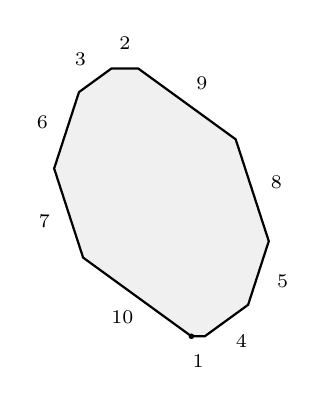
\begin{tikzpicture}[scale=0.17]
  \draw[thick, fill=gray!12] (0.000,0.000) -- (1.000,0.000) -- (4.236,2.351) -- (5.781,7.106) -- (3.309,14.715) -- (-3.972,20.005) -- (-5.972,20.005) -- (-8.399,18.242) -- (-10.253,12.535) -- (-8.090,5.878) -- cycle;
  \fill (0,0) circle (6pt);
  \node[font=\scriptsize] at (0.50,-1.90) {$1$};
  \node[font=\scriptsize] at (3.73,-0.36) {$4$};
  \node[font=\scriptsize] at (6.82,4.14) {$5$};
  \node[font=\scriptsize] at (6.35,11.50) {$8$};
  \node[font=\scriptsize] at (0.79,18.90) {$9$};
  \node[font=\scriptsize] at (-4.97,21.90) {$2$};
  \node[font=\scriptsize] at (-8.30,20.66) {$3$};
  \node[font=\scriptsize] at (-11.13,15.98) {$6$};
  \node[font=\scriptsize] at (-10.98,8.62) {$7$};
  \node[font=\scriptsize] at (-5.16,1.40) {$10$};
\end{tikzpicture}
\end{minipage}\hfill
\begin{minipage}[c]{0.66\textwidth}
\caption{The equiangular decagon of Theorem~\ref{thm:main}, sides labelled by their lengths. From the marked vertex $P_0=0$, counterclockwise, the sides are $1,4,5,8,9,2,3,6,7,10$; the vertices are $P_j=\sum_{k<j}s_k\zeta^k$ with $\zeta=e^{2\pi i/10}$, and every interior angle is $144^\circ$.}
\label{fig:decagon}
\end{minipage}
\end{figure}

\section{Statement}\label{sec:statement}

\subsection*{The OEIS conjecture}
The comments of A215010 contain the following sentence, verbatim:
\begin{quote}
Conjecture: hexagons are the only simple convex polygons with equal interior angles with such property, due to the fact that cos(Pi/3) = 1/2.
\end{quote}
The comment carries no separate attribution; the entry is by Robin Garcia, July~31, 2012.
``Such property'' refers to the entry's name: integer side lengths that are the terms $t+md$ of an arithmetic progression.

\subsection*{Mathematical formulation}
\begin{definition}\label{def:E}
For $N\in\N$ and $s\colon\{0,\dots,N-1\}\to\N$, write $\Eq_N(s)$ if $N\ge3$, $s_k>0$ for all $k$, and $\sum_{k=0}^{N-1}s_k\,e^{2\pi ik/N}=0$ in $\C$.
\end{definition}

\begin{remark}[Encoding of polygons]\label{rem:encoding}
For $N\ge3$ and $s_0,\dots,s_{N-1}>0$, a simple convex polygon with equal interior angles and consecutive sides $s_0,\dots,s_{N-1}$ (counterclockwise) exists if and only if \eqref{eq:close} holds with $\zeta=e^{2\pi i/N}$.
Indeed, the exterior angles of such a polygon are equal and sum to $2\pi$, so after a rotation the $k$th edge vector is $s_k\zeta^k$, and the polygon closes.
Conversely, if \eqref{eq:close} holds, the closed path $P_j=\sum_{k<j}s_k\zeta^k$ ($0\le j\le N$, $P_N=P_0$) has edge directions $\zeta^k$ whose arguments $2\pi k/N$ increase strictly through one full turn, so it turns left by $2\pi/N\in(0,\pi)$ at every vertex and bounds a convex polygon, traversed once, with all interior angles $\pi-2\pi/N$.
This equivalence justifies the encoding; the formal proof works with Definition~\ref{def:E} only.
\end{remark}

\begin{theorem}\label{thm:main}
Let $\sigma=(\sigma(0),\dots,\sigma(9))=(0,3,4,7,8,1,2,5,6,9)$ and $s_k=1+\sigma(k)\cdot1$, so that $(s_0,\dots,s_9)=(1,4,5,8,9,2,3,6,7,10)$.
Then $\sigma$ is a permutation of $\{0,\dots,9\}$ and $\Eq_{10}(s)$ holds.
Consequently, it is false that for all $N,t,d\in\N$ with $d\ge1$ and every permutation $\sigma$ of $\{0,\dots,N-1\}$, $\Eq_N(k\mapsto t+\sigma(k)d)$ implies $N=6$.
\end{theorem}

\subsection*{Lean statement}
The statement is the definition \decl{Math0.Statements.A215010.statement} in the frozen math0 statement file \path{lean/Math0/Statements/OEIS/A215010.lean}.
Its definitions are, verbatim (docstrings omitted; namespace \decl{Math0.Statements.A215010}):
\begin{lstlisting}
noncomputable def edgeDir (N k : ℕ) : ℂ := Complex.exp (2 * Real.pi * Complex.I * k / N)

def IsEquiangularPolygon (N : ℕ) (s : Fin N → ℕ) : Prop :=
  3 ≤ N ∧ (∀ k, 0 < s k) ∧ ∑ k : Fin N, (s k : ℂ) * edgeDir N k = 0

def statement : Prop :=
  ∀ (N t d : ℕ), 1 ≤ d → ∀ σ : Equiv.Perm (Fin N),
    IsEquiangularPolygon N (fun k => t + (σ k : ℕ) * d) → N = 6
\end{lstlisting}
Here \texttt{edgeDir N k} is $e^{2\pi ik/N}$, \texttt{IsEquiangularPolygon N s} is $\Eq_N(s)$, and \decl{statement} is the universal claim negated in Theorem~\ref{thm:main}; we prove \texttt{¬ statement}.

\subsection*{Encoding}
Polygons are encoded by Definition~\ref{def:E} (Remark~\ref{rem:encoding}); $N\ge3$ excludes $N=0$, where the closing condition would hold vacuously, and $N=1,2$.
The $N$ sides are $t,t+d,\dots,t+(N-1)d$ in the order given by $\sigma$; a negative difference gives the same set of sides, and positivity of the sides forces $t\ge1$.
The case $d=0$ is excluded, since regular polygons exist for every $N$ and would make the statement trivially false; the entry's solutions have distinct sides.
``Only'' is read as the claim that every such polygon has $N=6$; that hexagons have the property is the content of the sequence.
The only coercions are from $\mathrm{Fin}\,N$ to $\N$, from $\N$ to $\C$, and from $\mathbb{R}$ to $\C$ (for $\pi$), and \decl{statement} contains no subtraction or division in $\N$.

\subsection*{Check against the OEIS data}
The statement file computes the sequence from its definition, without hardcoding the terms.
The function \decl{lexPerms} lists the $720$ orderings $m$ of $0,\dots,5$ in lexicographic order, and \decl{primitiveSolutions} keeps those that pass two Boolean tests.
The first, \decl{hexCloses}, says $\sum_k m_k\omega^k=0$ for $\omega=e^{i\pi/3}$ as two integer dot products with the vectors $(2\operatorname{Re}\omega^k)_k=(2,1,-1,-2,-1,1)$ and $((2/\sqrt3)\operatorname{Im}\omega^k)_k=(0,1,1,0,-1,-1)$; as noted above, $t$ and $d$ drop out of \eqref{eq:close}.
The second, \decl{normalForm}, is the entry's normalization up to rotation and reflection: start at the shortest side ($m_0=0$) and go toward the longer neighbour ($m_1>m_5$), as in the entry's comment, which rewrites $(2,6,4,5,3,7)$ as $(2,7,3,5,4,6)$.
The sequence \decl{a} concatenates the surviving patterns (offset $1$, and $0$ outside $1,\dots,12$).
The kernel checks, by \texttt{decide +kernel}, the theorems \decl{a_data} ($a(1),\dots,a(12)$ are the $12$ listed terms) and \decl{primitiveSolutions_length} (there are exactly two patterns, so no further terms); both use only the axiom \decl{propext}.
The theorem \decl{hexCloses_iff} proves that for every $m\colon\mathrm{Fin}\,6\to\N$ the sum $\sum_k m_k\cdot\texttt{edgeDir 6 k}$ vanishes if and only if \texttt{hexCloses (List.ofFn m)} holds, tying the data check to the predicate in \decl{statement}; an \texttt{example} checks the entry's hexagon $(1,6,2,4,3,5)$ against \texttt{IsEquiangularPolygon 6}.

\section{Proof}\label{sec:proof}

Throughout, $\zeta=e^{2\pi i/10}$; in Lean, $\zeta$ is \texttt{edgeDir 10 1}.
The proof follows the auxiliary declarations of the Lean file: the permutation \texttt{σ10}, the lemmas \decl{zeta_props} and \decl{edgeDir_ten}, and the theorem \decl{decagon}.

\begin{lemma}[\decl{zeta_props}]\label{lem:zeta}
$\zeta^5=-1$ and $\Phi_{10}(\zeta)=\zeta^4-\zeta^3+\zeta^2-\zeta+1=0$.
\end{lemma}

\begin{proof}
The number $\zeta$ is a primitive $10$th root of unity; in Lean this is Mathlib's \decl{Complex.isPrimitiveRoot_exp}, after identifying \texttt{edgeDir 10 1} with $e^{2\pi i/10}$ by normalizing the exponent.
Since $5\mid10$, $\zeta^5$ is a primitive square root of unity (\decl{IsPrimitiveRoot.pow_of_dvd}), hence $\zeta^5=-1$ (\decl{IsPrimitiveRoot.eq_neg_one_of_two_right}).
Next, $\zeta+1\ne0$: otherwise $\zeta=-1$ and $\zeta^2=1$, contradicting primitivity since $0<2<10$ (\decl{IsPrimitiveRoot.pow_ne_one_of_pos_of_lt}).
Finally, $(x+1)(x^4-x^3+x^2-x+1)=x^5+1$ gives $(\zeta+1)\Phi_{10}(\zeta)=\zeta^5+1=0$, and $\zeta+1\ne0$ yields $\Phi_{10}(\zeta)=0$.
\end{proof}

\begin{lemma}[\decl{edgeDir_ten}]\label{lem:pow}
For every $k\in\N$, $e^{2\pi ik/10}=\zeta^k$.
\end{lemma}

\begin{proof}
$\zeta^k=\exp(2\pi i/10)^k=\exp(k\cdot 2\pi i/10)$ (\decl{Complex.exp_nat_mul}), and $k\cdot2\pi i/10=2\pi ik/10$.
\end{proof}

\begin{proposition}[\decl{decagon}]\label{prop:decagon}
With $s$ as in Theorem~\ref{thm:main}, $\Eq_{10}(s)$ holds.
\end{proposition}

\begin{proof}
We have $10\ge3$ and $s_k\ge1>0$ for every $k$.
By Lemma~\ref{lem:pow}, the closing sum is
\[
  S=\sum_{k=0}^{9}s_k\zeta^k = 1+4\zeta+5\zeta^2+8\zeta^3+9\zeta^4+2\zeta^5+3\zeta^6+6\zeta^7+7\zeta^8+10\zeta^9 .
\]
By Lemma~\ref{lem:zeta}, $\zeta^{5+j}=-\zeta^j$ for $j=0,\dots,4$.
In $\Z[x]$ we have the identity
\[
  \sum_{k=0}^{9}s_kx^k
  = -\Phi_{10}(x) + 2(x^5+1) + 3(x^6+x) + 6(x^7+x^2) + 7(x^8+x^3) + 10(x^9+x^4),
\]
since on the right the coefficients of $x^5,\dots,x^9$ are $2,3,6,7,10=s_5,\dots,s_9$ and those of $x^0,\dots,x^4$ are $-1+2,\,1+3,\,-1+6,\,1+7,\,-1+10=s_0,\dots,s_4$.
At $x=\zeta$ every term on the right vanishes, so $S=0$.
Equivalently, folding with $\zeta^{k+5}=-\zeta^k$ gives $S=\sum_{k<5}(s_k-s_{k+5})\zeta^k=-1+\zeta-\zeta^2+\zeta^3-\zeta^4=-\Phi_{10}(\zeta)=0$.
\end{proof}

In Lean, \texttt{simp} with \decl{Fin.sum_univ_succ} and the definition of \texttt{σ10} expands the sum into its ten terms, \texttt{norm\_num} normalizes the numerals, and \texttt{linear\_combination} with coefficients $-1,2,3,6,7,10$ applied to $\Phi_{10}(\zeta)=0$ and $\zeta^{5+j}=-\zeta^j$ checks the identity above by ring normalization.

\begin{proof}[Proof of Theorem~\ref{thm:main}]
The map $\sigma$ has the inverse $\tau=(0,5,6,1,2,7,8,3,4,9)$; in Lean, \texttt{σ10} is the permutation with these two vectors as maps $\mathrm{Fin}\,10\to\mathrm{Fin}\,10$, and both inverse identities are checked by \texttt{decide} on all ten inputs.
The claim $\Eq_{10}(s)$ is Proposition~\ref{prop:decagon}.
If the universal statement held, then applying it with $N=10$, $t=1$, $d=1\ge1$ and $\sigma$ would give $10=6$, which is false.
\end{proof}

\begin{remark}[Minimality and other counterexamples; not formalized]\label{rem:minimal}
By Remark~\ref{rem:encoding}, Theorem~\ref{thm:main} gives a simple convex decagon with interior angles $144^\circ$ and sides $1,4,5,8,9,2,3,6,7,10$ in counterclockwise order (Figure~\ref{fig:decagon}); the sides $t+(s_k-1)d$ give one for every $t,d\ge1$.
No counterexample has $N<10$: the values $N\in\{3,4,5,7,8,9\}$ are prime powers, and the following standard argument, in the spirit of Clark's result recorded in A118887, excludes them.
Let $N=p^a$, $M=p^{a-1}$, $\zeta_N=e^{2\pi i/N}$, and suppose $\sum_k(t+\sigma(k)d)\zeta_N^k=0$ with $d\ge1$.
Since $\sum_k\zeta_N^k=0$, the polynomial $f(x)=\sum_{k<N}\sigma(k)x^k$ vanishes at $\zeta_N$, so it is divisible in $\Q[x]$ by the minimal polynomial $\Phi_N(x)=\sum_{j<p}x^{jM}$ of $\zeta_N$, which has degree $N-M$.
Write $f=\Phi_N g$ with $g=\sum_{r<M}g_rx^r$; then $f=\sum_{j<p}\sum_{r<M}g_rx^{jM+r}$ with distinct exponents, so $\sigma(jM+r)=g_r$ for all $j,r$, and $\sigma(0)=\sigma(M)$ contradicts injectivity.
So $N=10$, the least $N\ne6$ that is not a prime power, is the least possible counterexample.
An independent enumeration (not part of the formal proof) finds $48$ orderings of $1,\dots,10$ with $s_0=1$ that satisfy \eqref{eq:close}, that is, $24$ up to reflection, in agreement with $a(10)=24$ in A118887.
\end{remark}

\section{Machine verification}\label{sec:lean}

\subsection*{Files and declarations}
The proof is in the file \path{lean/Math0/Frontier/OEIS/A215010.lean} of the math0 repository, \url{https://github.com/Foundation-0/math0}.
It imports the frozen statement file \path{lean/Math0/Statements/OEIS/A215010.lean} (Section~\ref{sec:statement}; SHA-256 \texttt{740251a2\ldots e40a}, unchanged since the fidelity review) and the audit commands in \path{lean/Math0/Audit.lean}.
The main declaration is \decl{Math0.Frontier.A215010.result}, of type \texttt{¬ Math0.Statements.A215010.statement}; the auxiliary declarations \texttt{σ10}, \decl{zeta_props}, \decl{edgeDir_ten} and \decl{decagon} are private.
The proof file is, verbatim except for the license header, the imports, the docstrings and blank lines:
\begin{lstlisting}[basicstyle=\ttfamily\scriptsize]
namespace Math0.Frontier.A215010
open Math0.Statements.A215010
private def σ10 : Equiv.Perm (Fin 10) where
  toFun := ![0, 3, 4, 7, 8, 1, 2, 5, 6, 9]
  invFun := ![0, 5, 6, 1, 2, 7, 8, 3, 4, 9]
  left_inv := by decide
  right_inv := by decide
private theorem zeta_props :
    edgeDir 10 1 ^ 4 - edgeDir 10 1 ^ 3 + edgeDir 10 1 ^ 2 - edgeDir 10 1 + 1 = 0 ∧
      edgeDir 10 1 ^ 5 = -1 := by
  have hz : IsPrimitiveRoot (edgeDir 10 1) 10 := by
    have := Complex.isPrimitiveRoot_exp 10 (by norm_num)
    unfold edgeDir
    convert this using 2
    push_cast; ring
  set ζ := edgeDir 10 1
  have h5 : ζ ^ 5 = -1 := by
    have h2 : IsPrimitiveRoot (ζ ^ 5) (10 / 5) := hz.pow_of_dvd (by norm_num) (by norm_num)
    exact IsPrimitiveRoot.eq_neg_one_of_two_right h2
  have hne : ζ + 1 ≠ 0 := by
    intro h
    have : ζ = -1 := by linear_combination h
    have h2 : ζ ^ 2 ≠ 1 := hz.pow_ne_one_of_pos_of_lt (by norm_num) (by norm_num)
    exact h2 (by rw [this]; norm_num)
  refine ⟨?_, h5⟩
  have hprod : (ζ + 1) * (ζ ^ 4 - ζ ^ 3 + ζ ^ 2 - ζ + 1) = 0 := by
    linear_combination h5
  exact (mul_eq_zero.mp hprod).resolve_left hne
private theorem edgeDir_ten (k : ℕ) : edgeDir 10 k = edgeDir 10 1 ^ k := by
  unfold edgeDir
  rw [← Complex.exp_nat_mul]; congr 1; push_cast; ring
private theorem decagon : IsEquiangularPolygon 10 (fun k => 1 + (σ10 k : ℕ) * 1) := by
  refine ⟨by norm_num, fun _ => by positivity, ?_⟩
  obtain ⟨hΦ, h5⟩ := zeta_props
  rw [Finset.sum_congr rfl fun k _ => by rw [edgeDir_ten]]
  set ζ := edgeDir 10 1
  simp [Fin.sum_univ_succ, σ10]
  have h6 : ζ ^ 6 = -ζ := by linear_combination ζ * h5
  have h7 : ζ ^ 7 = -ζ ^ 2 := by linear_combination ζ ^ 2 * h5
  have h8 : ζ ^ 8 = -ζ ^ 3 := by linear_combination ζ ^ 3 * h5
  have h9 : ζ ^ 9 = -ζ ^ 4 := by linear_combination ζ ^ 4 * h5
  norm_num
  linear_combination (-1 : ℂ) * hΦ + 2 * h5 + 3 * h6 + 6 * h7 + 7 * h8 + 10 * h9
theorem result : ¬ statement := by
  intro h
  have := h 10 1 1 le_rfl σ10 decagon
  norm_num at this
end Math0.Frontier.A215010
#math0_settles Math0.Frontier.A215010.result Math0.Statements.A215010.statement
\end{lstlisting}
The proof file uses no \texttt{sorry}, \texttt{native\_decide} or \texttt{set\_option}; its only uses of \texttt{decide} are the two ten-case checks for \texttt{σ10}.
The data checks of Section~\ref{sec:statement} live in the statement file; \decl{result} does not depend on them.

\subsection*{Audit}
The command \texttt{\#math0\_settles} (in \path{lean/Math0/Audit.lean}, for statements that math0 formalizes itself) fails unless \decl{statement} is a \texttt{Prop}-valued definition without universe parameters, both \decl{statement} and \decl{result} use no axioms besides \decl{propext}, \decl{Classical.choice} and \decl{Quot.sound} (this rejects \decl{sorryAx}, the axiom \decl{Lean.ofReduceBool} introduced by \texttt{native\_decide}, and custom axioms), and the type of \decl{result} is syntactically the statement or its negation, up to metadata annotations, with no unfolding.
Running \texttt{lake env lean Math0/Frontier/OEIS/A215010.lean} in the directory \path{lean} prints
\begin{lstlisting}[basicstyle=\ttfamily\scriptsize]
math0 audit: 'Math0.Statements.A215010.statement' depends on axioms [Classical.choice, Quot.sound, propext]
math0 audit: 'Math0.Frontier.A215010.result' depends on axioms [Classical.choice, Quot.sound, propext]
math0 statement check: 'Math0.Frontier.A215010.result' refutes 'Math0.Statements.A215010.statement'
\end{lstlisting}
so \decl{result} proves the negation of the statement and depends only on the three standard axioms; the statement itself uses \decl{Classical.choice} and \decl{Quot.sound} through Mathlib's construction of $\mathbb{R}$ and $\C$.

\subsection*{Toolchain and reproduction}
We use Lean~4 \cite{Lean4} \texttt{v4.33.1} and Mathlib \cite{Mathlib} \texttt{v4.33.1}, pinned in \path{lean/}; the repository also pins formal-conjectures \cite{FC} at commit \texttt{c77fdd4}, which this result does not use.
To reproduce, run \path{scripts/verify.sh} from the repository root: it fetches the Mathlib build cache, builds all math0 results with \texttt{lake build} (re-running every audit command), checks that the pinned \texttt{formal\_conjectures} and \texttt{mathlib} checkouts are unmodified, and reports the number of passed statement checks.
To check this result alone, run \texttt{lake build Math0.Statements.OEIS.A215010} and then \texttt{lake env lean Math0/Frontier/OEIS/A215010.lean} in the directory \path{lean}; on our machine the second command takes well under a minute of wall time (about $22$ seconds in our last run), most of it spent loading Mathlib.

{\small
\begin{thebibliography}{99}

\bibitem{Abel}
U.~Abel, \emph{Coincidence of the barycentre and the geometric centre of weighted points}, Math. Gaz. \textbf{103} (2019), no.~558, 409--415, doi:10.1017/mag.2019.101.

\bibitem{Ball}
D.~Ball, \emph{Equiangular polygons}, Math. Gaz. \textbf{86} (2002), no.~507, 396--407, doi:10.2307/3621131.

\bibitem{Bernoff}
A.~Bernoff, \emph{Bernoff's Puzzler}, MuddMath Newsletter \textbf{4} (Spring 2005), no.~1, p.~10, Harvey Mudd College.

\bibitem{FC}
M.~Firsching, P.~Lezeau, S.~Mercuri, M.~Z. Horv\'ath, Y.~Dillies, C.~S\"onne, E.~Wieser, F.~Zhang, T.~Hubert, B.~Ag\"uera y Arcas, and P.~Kohli, \emph{Formal Conjectures: An Open and Evolving Benchmark for Verified Discovery in Mathematics}, arXiv:2605.13171, 2026. Repository: \url{https://github.com/google-deepmind/formal-conjectures}.

\bibitem{Mathlib}
The mathlib Community, \emph{The Lean mathematical library}, in: Proceedings of the 9th ACM SIGPLAN International Conference on Certified Programs and Proofs (CPP 2020), ACM, 2020, 367--381.

\bibitem{Lean4}
L.~de Moura and S.~Ullrich, \emph{The Lean 4 theorem prover and programming language}, in: Automated Deduction -- CADE 28, Lecture Notes in Comput. Sci. \textbf{12699}, Springer, 2021, 625--635.

\bibitem{Munteanu}
M.~Munteanu and L.~Munteanu, \emph{Rational equiangular polygons}, Applied Math. \textbf{4} (2013), no.~10, 1460--1465, doi:10.4236/am.2013.410197.

\bibitem{A118887}
The OEIS Foundation Inc., \url{https://oeis.org/A118887}, entry by H.~Pfoertner, May~3, 2006; revision \#45, Mar.~19, 2026.

\bibitem{A215010}
The OEIS Foundation Inc., \url{https://oeis.org/A215010}, entry by R.~Garcia, Jul.~31, 2012; revision \#43, Jan.~23, 2015.

\bibitem{Woeginger}
G.~J. Woeginger, \emph{Nothing new about equiangular polygons}, Amer. Math. Monthly \textbf{120} (2013), no.~9, 849--850, doi:10.4169/amer.math.monthly.120.09.849.

\end{thebibliography}
}

\end{document}
